\documentclass[a4paper,UTF8]{article}
\usepackage{graphics}
\usepackage{xeCJK}
\usepackage{fancyhdr}
\usepackage{indentfirst}
\usepackage{amsmath}
\usepackage{float}

\newCJKfontfamily[kaiti]\kaiti{KaiTi}

\newcommand{\yihao}{\fontsize{26pt}{36pt}\selectfont}           % 一号, 1.4 倍行距
\newcommand{\erhao}{\fontsize{22pt}{28pt}\selectfont}          % 二号, 1.25倍行距
\newcommand{\xiaoer}{\fontsize{18pt}{18pt}\selectfont}          % 小二, 单倍行距
\newcommand{\sanhao}{\fontsize{16pt}{24pt}\selectfont}        % 三号, 1.5倍行距
\newcommand{\xiaosan}{\fontsize{15pt}{22pt}\selectfont}        % 小三, 1.5倍行距
\newcommand{\sihao}{\fontsize{14pt}{21pt}\selectfont}            % 四号, 1.5 倍行距
\newcommand{\banxiaosi}{\fontsize{13pt}{19.5pt}\selectfont}    % 半小四, 1.5倍行距
\newcommand{\xiaosi}{\fontsize{12pt}{18pt}\selectfont}            % 小四, 1.5倍行距
\newcommand{\dawuhao}{\fontsize{11pt}{11pt}\selectfont}       % 大五号, 单倍行距
\newcommand{\wuhao}{\fontsize{10.5pt}{15.75pt}\selectfont}    % 五号, 单倍行距

\pagestyle{fancy}
\fancyhf{}
\lhead{
\includegraphics{figure/sjtubanner}}
\chead{}
\rhead{船舶设备2018}%需修改之处
\lfoot{}
\cfoot{\small --~~{\bfseries\thepage}~~of~~{\bfseries{\pageref{last}}}~~--}
\rfoot{}
\fancyheadoffset{50pt}
\renewcommand{\headheight}{32pt}

\setlength{\parindent}{2.45em}%来调整首行缩进的大小。这里的 2.45em 是中文小四号字大小两个中文字的长度。

\begin{document}
\begin{titlepage}
	\thispagestyle{empty}
	\begin{center}
		\vspace*{20pt} \vskip 7pt
		
\includegraphics{figure/sjtulogo}
		\vskip 30pt
		{\kaiti \fontsize{32}{32} 舵设备大作业}%修改之处
		\vskip 15pt 
		{\xiaosi \MakeUppercase{\textbf{Ship Equipment Project--Rudder}}}
		\vskip 15pt
		
\includegraphics{figure/sjtubadge}
		\vskip \stretch{2}
		    \vskip \stretch{1}
		{\kaiti\sanhao
			\def\arraystretch{1.1}
			\begin{tabular}{r@{:}l}%修改之处
				\makebox[4em][s]{学生姓名}        & \underline{\makebox[180pt]{简心语}} \\
				\makebox[4em][s]{学生学号} 		& \underline{\makebox[180pt]{515021910260}} \\
				\makebox[4em][s]{指导老师}        & \underline{\makebox[180pt]{赵永生}} \\
				\makebox[4em][s]{专\hspace{\fill}业}    	      & \underline{\makebox[180pt]{船舶与海洋工程}} \\
				\makebox[4em][s]{学\hspace{\fill}院}     & \underline{\makebox[180pt]{船舶海洋与建筑工程学院}}
		\end{tabular}}
	\end{center}
\end{titlepage}

\newpage
\tableofcontents
\newpage
\section{船况概述}
本船为一艘自航绞吸式挖泥船,主要用于我国长江中、上游航道维护清淤、疏浚等施工作业。设计作业水域主要为长江中、上游,包括三线库尾水域,航行区域为长江和三峡库区,包括A、B级和J2级急流航段.
该船的主尺度见表\ref{tab:zcd}:
\begin{table}[!htbp]
	\centering
	\begin{tabular}{ccc}

		\hline 
		主尺度 & 符号 & 数值\\
		\hline
		总长 & $L_{OA}$ & 93.10m\\
		垂向间长 & $L_{PP}$ & 89.90m\\
		型宽 & $B$ & 23.00m\\
		型深	& $D$ & 5.30m\\
		设计吃水 & $d$ & 3.40m\\
		载重线吃水 & $d_s$ & 4.10m\\
		设计吃水排水量 & $\Delta$ & 5568.08t\\
		载重线吃水排水量 & $\Delta_S$ & 6789.53t\\
		船员人数	& & 30P\\
		设计航速(设计吃水时) & & 19.2$km/h$\\
		\hline
	\end{tabular}
	\caption{$JD9115-100-01SM$主尺度}
	\label{tab:zcd}
\end{table}
螺旋桨主要要素见表\ref{tab:propeller}:
\begin{table}[!htbp]
	\centering
	\begin{tabular}{ccc}
		\hline
		螺旋桨直径 & D & 2.19m \\
		型式 & JD75+Ka 4 & \\
		螺旋桨转速 & N & 250r/min \\
		有效系柱推力 & Te & 22982 kgf\\
		最大计算航速 & V & 10.38 kn\\
		螺旋桨伴流系数 & $\psi_{S}$ & 0.3\\
		\hline	
	\end{tabular}
\caption{螺旋桨主要要素}
\label{tab:propeller}
\end{table}

\section{舵的基本参数}
\subsection{设计理念}

\subsection{数量}
由于该船为内河船,吃水较浅且作为工程船有着较高的操纵性要求,同时由于该船配备了双螺旋桨,决定采用%双导管襟翼舵
双流线型舵.虽然对于处在长江上游急流航段,操纵性要求高的挖泥船,配置双桨三舵似乎是更好的选择,但考虑到装配难度和成本,此处不予考虑.
\subsection{位置}
舵与螺旋桨的纵向距离一般不应妨碍螺旋桨拆装要求,纵向距离一般为$1/4~1/2D$(D—螺旋桨直径). 舵叶中心大多与螺旋桨中心的垂向距离二者接近一致为佳, 若有偏移在$0.1D$范围内. 以及一般舵设备的设计都是在船舶型线设计之后进行的, 因此, 舵叶的布置将受到尾部线型的限制. 根据舵的布置原则:
\begin{enumerate}
	\item 从侧面看, 舵叶上缘不可超出设计水线并应与尾部线型有良好的吻合, 舵上缘与船底间隙尽量小, 可利用边界效应提高舵效.
	\item 舵的下缘不得超出船底基线, 使得舵受到船体遮蔽保护, 以避免损伤, 一般留有200mm间隙.
	\item 舵的前缘与螺旋桨的距离还需注意螺旋桨和尾轴的安装和拆卸的工艺要求.
	\item 从水平面看, 在任何可能达到的舵角下, 舵叶均不应超出船尾轮廓线.
	\item 将舵布置在尾流速度大处工作, 以提高舵效.
	\item 舵应布置在远离船舶重心处, 以便增大转船力臂.
\end{enumerate}

\subsection{型式,侧面形状}
考虑到本船为内河工程船, 对于操纵性的要求较高. 而悬挂舵常用于在双桨近海调查船和作业船舶, 该船的工作环境, 类似于近海作业船舶.故采用悬挂舵的方式. 

考虑到工艺性, 舵外形常为矩形, 且对悬挂舵一般取倒梯形.
\subsection{舵面积}
首先按《船舶设计实用手册-舾装分册》(以下简称手册)中的表1.1.4.2,机动性较高的船舶舵面积比的范围为$2.0~4.0$.???
其次根据DNV《船舶入级规范》关于舵面积的规定,直接在推进器后面工作的单舵或多舵,其舵面积应不小于式\ref{equ:dnv}所得值.
\begin{equation}\label{equ:dnv}
\begin{split}
&A = \frac{dL}{100}[1+50C^{2}_{B}(\frac{B}{L})^{2}]\\
&C_{B}=\frac{\Delta}{1.025LBd}
\end{split}
\end{equation}
将本船的船型参数带入公式,可以计算得到最小的舵面积比为:$2.956\%$.对于在狭窄水道内频繁地机动航行地船舶,舵面积应予增加,于是取舵面积比$\chi=3.6\%$(待修正). 由式\ref{equ:rarea}得舵面积$A_{R}=11.00376 m^{2}$,故单个舵的面积$A=5.50188 m^{2}$. 结合尾部线型的限制, 取舵面积比$\chi=3.557111\%$, 舵面积$A_{R}=10.872664 m^{2}$, 单个舵的面积$A=5.436332 m^{2}$.
\begin{equation}\label{equ:rarea}
A_{R} = \chi L_{PP}d
\end{equation}

\subsection{展弦比}
综合以上, 确定舵宽(梯形中位线)$b_{m}=1740 mm$, 舵高$h_{m}=3200 mm$.展弦比$\lambda=\frac{h_{m}}{b_{m}}=1.839080$\\

\subsection{平衡系数}
平衡系数$e=\frac{A_{R}}{A_{C}}$, 其中$A_{C}$为舵转轴前部分舵面积. 实际设计中, 舵平衡系数的选定需要考虑到与船体、螺旋桨等的配合, 常在$0.2~0.3$之间. 综合考虑, 不妨取定$e=0.26$
\subsection{舵的初步设计}
舵的初步设计如图\ref{fig:r1}所示. 舵的上缘与尾部线性有良好吻合, 间隙不大.舵的前缘与螺旋桨的距离约为$0.25D$, 舵叶中心与螺旋桨中心的垂向距离约为$0.094D$, 舵的下缘距船底基线$200mm$, 舵面积$A=5.436332 m^{2}$, 舵平衡系数待定$e=0.256961$. 总体符合要求.
\begin{figure}
	\centering
	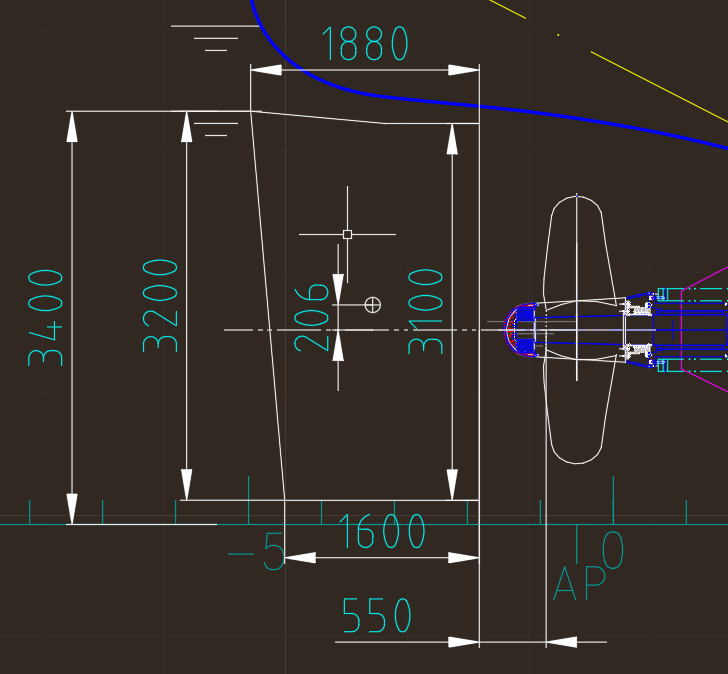
\includegraphics[width=3.5in]{figure/RUDDER-V1}
	\caption{Rudder V1.0}
	\label{fig:r1}
\end{figure}

\section{水动力特性计算}
\subsection{舵叶剖面翼型}
选用应用最广泛的NACA0015,对称剖面,厚度比$\bar{t}=15\%$.舵的厚度$t=\bar{t}b_{m}=225mm$.
\subsection{理论计算}
舵的水动力计算采用模型试验资料是最接近实际的方法.这些资料通常有: 自航模型
试验资料、舵的模型试验资料以及单独舵的图谱资料. 这里采用单独舵的图谱资料.根据《船舶设计实用手册-舾装分册》表1.1.4.3 $\lambda=1.0$的舵的水动力特性(正车时)及表1.1.4.4 $\lambda=1.0$的舵的水动力特性(倒车时), 可得NACA0015在$Re=0.79\times 10^6$时不同攻角$\alpha$下的升力系数$C_{y}(\alpha)$, 法向力系数$C_{n}(\alpha)$, 力矩系数$C_{m0.25}$的值. 再根据式\ref{equ:c}计算出阻力系数$C_{x}$, 压力中心系数$C_{p}$,力矩系数$C_{m0}$.
\begin{equation}\label{equ:c}
\begin{split}
&	C_{x}=\frac{C_{n}-C_{y}cos\alpha}{sin\alpha}\\
&C_{p}=\frac{C_{m0.25}}{C_{n}}+0.25\\
&C_{m0}=C_{m0.25}+0.25C_{n}
\end{split}
\end{equation}
因舵的实际展弦比$\lambda=1.839080$, 故需按Prandtl公式(式\ref{equ:prandtl})进行换算.
\begin{equation}\label{equ:prandtl}
\begin{split}
&\alpha_{2}=\alpha_{1}+57.3\frac{C_{y1}}{\pi}(\frac{1}{\lambda_{2}}-\frac{1}{\lambda_{1}})\\
&C_{x2}=C_{x1}+\frac{C_{y1}^2}{\pi}(\frac{1}{\lambda_{2}}-\frac{1}{\lambda_{1}})\\
&C_{y2}=C_{y1}
\end{split}
\end{equation}
式中: 下标1表示模型舵, 下标2表示实船舵, $\alpha_{1}$,$\alpha_{2}$的单位均为度.\\
在流经舵叶的水流发生分离之前,可取$C_{p2}=C_{p1}$.\\
再由式\ref{equ:cn}计算出切向力系数$C_{n}$.
\begin{equation}\label{equ:cn}
C_{n}=C_{x}sin\alpha+C_{y}cos\alpha
\end{equation}
再由式\ref{equ:ct}计算出切向力系数$C_{t}$.
\begin{equation}\label{equ:ct}
	C_{t}=C_{x}cos\alpha-C_{y}sin\alpha
\end{equation}
最终得到各水动力系数,如表\ref{tab:zc}及表\ref{tab:dc}所示.

\begin{table}[htbp]
	\centering
	\begin{tabular}{cccccccc}
		\hline
		\multicolumn{1}{l}{$\alpha_{1}$} & \multicolumn{1}{l}{$\alpha_{2}$} & \multicolumn{1}{l}{$C_{x}$} & \multicolumn{1}{l}{$C_{y}$} & \multicolumn{1}{l}{$C_{n}$} & \multicolumn{1}{l}{$C_{t}$} & \multicolumn{1}{l}{$C_{m0}$} & \multicolumn{1}{l}{$C_p$} \\
		\hline
    5     & 3.63566 & 0.026216 & 0.141 & 0.142379 & 0.017222 & 0.021664 & 0.152098 \\
10    & 7.203586 & 0.030431 & 0.289 & 0.290535 & -0.00605 & 0.051731 & 0.178082 \\
15    & 10.73281 & 0.041406 & 0.441 & 0.440996 & -0.04145 & 0.091283 & 0.207207 \\
20    & 13.98142 & 0.076879 & 0.622 & 0.622147 & -0.07568 & 0.149328 & 0.240476 \\
25    & 17.50097 & 0.13191 & 0.775 & 0.778795 & -0.10726 & 0.198083 & 0.255031 \\
30    & 21.03986 & 0.195591 & 0.926 & 0.934485 & -0.1499 & 0.257907 & 0.277027 \\
35    & 28.10089 & 0.454338 & 0.713 & 0.842956 & 0.064938 & 0.330865 & 0.392052 \\
40    & 33.36215 & 0.536044 & 0.686 & 0.867742 & 0.070458 & 0.347413 & 0.399891 \\
45    & 38.89434 & 0.586796 & 0.631 & 0.859552 & 0.060509 & 0.34958 & 0.406319 \\
		\hline
	\end{tabular}
	\caption{舵的水动力特性(正车)}
	\label{tab:zc}
\end{table}

\begin{table}[htbp]
	\centering
	\begin{tabular}{cccccccc}
		\hline
		\multicolumn{1}{l}{$\alpha_{1}$} & \multicolumn{1}{l}{$\alpha_{2}$} & \multicolumn{1}{l}{$C_{x}$} & \multicolumn{1}{l}{$C_{y}$} & \multicolumn{1}{l}{$C_{n}$} & \multicolumn{1}{l}{$C_{t}$} & \multicolumn{1}{l}{$C_{m0}$} & \multicolumn{1}{l}{$C_p$}\\
		\hline
    5     & 2.668042 & 0.025035 & 0.241 & 0.241904 & 0.013789 & -0.01618 & -0.06687 \\
10    & 6.37024 & -0.78831 & 0.385 & 0.295157 & -0.82616 & -0.1122 & -0.38821 \\
15    & 9.984332 & -0.49266 & 0.532 & 0.438525 & -0.57744 & -0.13375 & -0.30919 \\
20    & 13.93783 & -0.18642 & 0.643 & 0.579166 & -0.33581 & -0.1504 & -0.26159 \\
25    & 17.73105 & -0.10233 & 0.771 & 0.703209 & -0.33228 & -0.16748 & -0.23988 \\
30    & 21.34514 & 0.00159 & 0.918 & 0.855608 & -0.33266 & -0.20199 & -0.23775 \\
35    & 25.36464 & 0.238541 & 1.022 & 1.025665 & -0.22226 & -0.1855 & -0.18167 \\
40    & 30.0158 & 0.518161 & 1.059 & 1.176179 & -0.08109 & -0.16618 & -0.14151 \\
45    & 35.47777 & 0.793467 & 1.01  & 1.283002 & 0.05996 & -0.13677 & -0.10652 \\
50    & 44.60721 & 1.365358 & 0.572 & 1.366042 & 0.570364 & 0.014669 & 0.01069 \\
		\hline
	\end{tabular}
	\caption{舵的水动力特性(倒车)}
	\label{tab:dc}
\end{table}

\subsection{修正计算}
自由水面与船底对于该船的影响可以忽略不计.
\subsubsection{船体的影响}
船体的伴流降低了舵的迎流速度, 因设计舵的上缘与船底的距离大部分大于舵的最大厚度225mm, 所以由手册表1.1.3.1得, 舵处的伴流系数可用式\ref{equ:banliu}计算得$\psi_{R}=0.412559$.
\begin{equation}\label{equ:banliu}
	\psi_{R}=(0.68C_{B}-0.43+\delta\psi+0.18\frac{2h_{1}+h_{2}}{H})u
\end{equation}
式中:巡洋舰尾船舶取$\delta\psi=0.18$,当舵布置在船体中心线的两侧时$u=C_{B}+0.15$.$h_{1}, h_{2}$的定义见图\ref{fig:h1h2}.\\
\begin{figure}
	\centering
	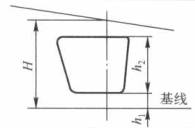
\includegraphics[width=1in]{figure/h1h2}
	\caption{$h_{1}, h_{2}$的定义}
	\label{fig:h1h2}
\end{figure}
舵的迎流速度由式\ref{equ:vr}得$v_{R}=3.133019$
\begin{equation}\label{equ:vr}
	v_{R}=v(1-\psi_{R})
\end{equation}
式中$v=19.2km/h=5.33m/s$为设计航速.
船体影响系数由式\ref{equ:kn}计算得$k_{n}=0.345087$
\begin{equation}\label{equ:kn}
	k_{n}=(1-\psi_{R})^2
\end{equation}
\subsubsection{螺旋桨的影响}
按照理想推进器理论,螺旋桨的迎流速度按式\ref{equ:vp}计算得$v_{P}=3.733333m/s$
\begin{equation}\label{equ:vp}
	v_{P}=v(1-\psi_{S})
\end{equation}
在舵的水动力计算中,通常按照理想推进器确定其轴向平均速度, 由式\ref{equ:vx}得螺旋桨后方尾流速度.
\begin{equation}\label{equ:vx}
\begin{split}
&v_{x}=v_{P}\sqrt{1+\sigma_{P}}=8.586546m/s\\
&\sigma_{P}=\frac{8P}{\pi\rho v_{P}^2D^2}=4.289852\\
&P = \frac{P_{e}}{1-\theta}
\end{split}
\end{equation}
式\ref{equ:vx}中$\sigma_{P}$为螺旋桨推力载荷系数(无因次值), $\rho$为水密度, 取$1000kg/m^3$, $P$为螺旋桨推力, $\theta$为推力减额系数. 这里$P$直接取为有效系柱推力$Te$, 由于是双桨, 故$P=22982kgf/2=112611.8N$.
\subsubsection{法向力及扭矩计算}
综合考虑船体和螺旋桨的影响.
\begin{equation}
\begin{split}
&k_{S}=1+\frac{A_{1}}{A}[(1+\sigma_{P})(\frac{1-\psi_{S}}{1-{\psi_{R}}})^2-1]\\
&N = C_{n}k_{n}k_{S}\frac{\rho v^2}{2}A\\
&M = C_{m}k_{n}k_{S}\frac{\rho v^2}{2}Ac
\end{split}
\end{equation}
式中$A_{1}$为处于螺旋桨尾流中的部分舵面积, 如图\ref{fig:a1}阴影部分所示,$A_{1}=3.791647m^2$, 计算得$k_{S}=5.541350$.\\
$C_{m}=C_{m0}$.\\在倒车计算时, 速度$v$应取正车时的一半.
由式\ref{equ:bh}计算得舵的水动压力中心到舵杆轴线的距离$b_{H}$.
\begin{equation}\label{equ:bh}
	b_{H}=(C_{P}-\beta)c
\end{equation}
式中:$C_{P}$--压力中心系数.\\
$\beta$--舵平衡系数, 由式\ref{equ:tfr}得$\beta=0.25$.\\
$c$--舵宽(m), 取平均宽度, 由式\ref{equ:tfr}得$c=1.74m$.
\begin{figure}
	\centering
	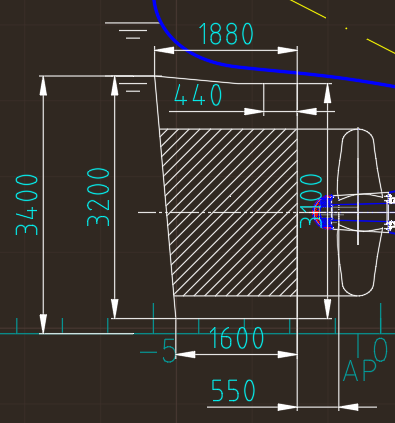
\includegraphics[width=3in]{figure/area1}
	\caption{螺旋桨尾流中的部分舵面积}
	\label{fig:a1}
\end{figure}
计算结果如表\ref{tab:zfxl}及表\ref{tab:dfxl}所示.
\begin{table}[htbp]
	\centering
	\begin{tabular}{ccccc}
		\hline
		\multicolumn{1}{l}{角度} & \multicolumn{1}{l}{转化角度} & \multicolumn{1}{l}{$b_{H}$} & \multicolumn{1}{l}{法向力N} & \multicolumn{1}{l}{扭矩M} \\
		\hline
    5     & 3.63566 & -0.17035 & 21024.2 & -509.924 \\
10    & 7.203586 & -0.12514 & 42901.52 & -1559.76 \\
15    & 10.73281 & -0.07446 & 65119.26 & -2138.28 \\
20    & 13.98142 & -0.01657 & 91868.74 & -947.155 \\
25    & 17.50097 & 0.008755 & 114999.9 & 784.0842 \\
30    & 21.03986 & 0.047027 & 137989.8 & 6064.104 \\
35    & 28.10089 & 0.24717 & 124474.3 & 25934.66 \\
40    & 33.36215 & 0.26081 & 128134.2 & 28998.73 \\
45    & 38.89434 & 0.271996 & 126924.8 & 29674.3 \\
		\hline
	\end{tabular}%
	\caption{正车时舵的法向力及扭矩}
	\label{tab:zfxl}
\end{table}

\begin{table}[htbp]
	\centering
	\begin{tabular}{ccccc}
		\hline
		\multicolumn{1}{l}{角度} & \multicolumn{1}{l}{转化角度} & \multicolumn{1}{l}{$b_{H}$} & \multicolumn{1}{l}{法向力N} & \multicolumn{1}{l}{扭矩M} \\
		\hline
    5     & 2.668042 & -0.55136 & 8930.131 & -1191.06 \\
10    & 6.37024 & -1.11049 & 10896.03 & -3571.38 \\
15    & 9.984332 & -0.973 & 16188.6 & -6907.42 \\
20    & 13.93783 & -0.89016 & 21380.5 & -11022.7 \\
25    & 17.73105 & -0.8524 & 25959.67 & -15560.6 \\
30    & 21.34514 & -0.84868 & 31585.63 & -22935.5 \\
35    & 25.36464 & -0.7511 & 37863.43 & -29169.2 \\
40    & 30.0158 & -0.68123 & 43419.82 & -34790.2 \\
45    & 35.47777 & -0.62035 & 47363.3 & -37696.8 \\
50    & 44.60721 & -0.4164 & 50428.8 & -28684.9 \\
		\hline
	\end{tabular}%
	\caption{倒车时舵的法向力及扭矩}
	\label{tab:dfxl}
\end{table}

\section{规范计算}
\subsection{舵力}
舵力$F(N)$按式\ref{equ:fn}计算.
\begin{equation}\label{equ:fn}
\begin{split}
&F=132K_{1}K_{2}K_{3}AV_{d}^2\\
&K_{1}=\frac{1}{3}(\lambda+2)\\
&\lambda=\frac{b^2}{A_{t}}\\
&b=\frac{1}{2}(Z_{3}+Z_{4}-Z_{2})
\end{split}
\end{equation}
式中:$b$--舵叶平均高度$(m)$, $Z_{2}$等的定义见图\ref{fig:aver}.计算得$b=3.150m$\\
$A_{t}$--舵面积$(m^2)$,对于无舵柱的舵即为舵叶面积$A=5.436332m^{2}$.\\
\\$\lambda$--展弦比取值不必大于2,计算得$\lambda=1.825220$. \\$K_{2}=1.1$(正车),$K_{2}=0.8$倒车. \\$K_{3}=1.0$. \\$V_{d}$--舵设计航速$(kn)$应按夏季载重吃水时船舶得最大营运航速$V$确定, 正车时,
\begin{equation}
\begin{split}
&V_{d}=V	(V>10kn)\\
&V_{d}=(V+20)/3 (V<10kn)
\end{split}
\end{equation}
倒车时,$V_{d}$应为最大倒车速度, 但取值应不小于$0.5V$. 因缺乏相关数据, 取$V_{d}=10.38kn$(正车), $V_{d}=5.19kn$(倒车).
计算出正车舵力108443.2333N, 倒车舵力19716.95151N.
对比理论计算结果, 最大正车舵力137472.1775N, 最大倒车舵力50658.23395N, 正车时二者较为接近, 倒车时差别较大.
\begin{figure}
	\centering
	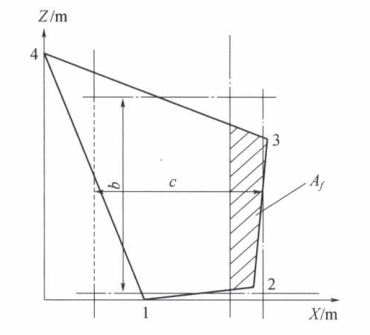
\includegraphics[width=2.5in]{figure/average}
	\caption{舵的平均高度和平均宽度计算图}
	\label{fig:aver}
\end{figure}

\subsection{舵杆扭矩}
船舶正车和倒车时的舵杆扭矩$T(N*m)$按下式计算.
\begin{equation}\label{equ:tfr}
\begin{split}
&T=FR\\
&	R=c(\alpha-\beta)\\
&c=\frac{1}{2}(X_{2}+X_{3}-X_{1})
\end{split}
\end{equation}
式中:$F$--舵力(N).\\$R$--无缺口舵叶力臂(m)\\$c$--舵叶平均宽度(m), $X_{1}$等的定义见图\ref{fig:aver}, 计算得$c=1.74m$\\
$\alpha$--压力中心系数, 正车0.33, 倒车0.66.\\
$\beta=\frac{A_{f}}{A}$--平衡系数, $A_{f}$为舵杆中心线前方的面积$(m^2)$, $A$为舵叶面积$(m^2)$, 见图\ref{fig:aver}, 计算得$\beta=0.25$.\\
得正车舵杆扭矩$15095.29808N\cdot m$, 倒车舵杆扭矩$14066.07321N\cdot m$.对比水动力计算得到的舵杆最大正车扭矩$89819.54456N\cdot m$, 最大倒车扭矩$12974.2937N\cdot m$. 可以发现, 正车差别较大, 倒车差别较小.

\subsection{舵杆-舵叶系统受力分析}
为了求得下舵承处的舵杆弯矩, 舵叶弯矩和剪力以及各轴承的支持力.
下舵承处的舵杆弯矩$M_{b}$:
\begin{equation}
\begin{split}
	M_{b}&=F[l_{2}+\frac{l_{1}(2C_{1}+C_{2})}{3(C_{1}+C_{2})}\\
		&=108443.2333\times[0.5+\frac{3.15\times(2\times 1.6+1.88)}{3\times(1.6+1.88)}]\\
		&220438.917 N\cdot m
\end{split}
\end{equation}
式中:$F$--舵力(N).\\其余各参数(m)定义见图\ref{fig:cal}.
\begin{figure}
	\centering
	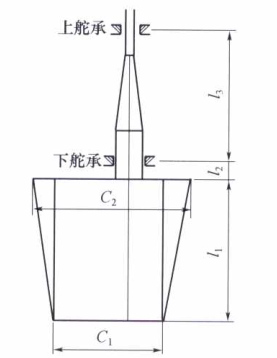
\includegraphics[width=2in]{figure/calculate}
	\caption{锥体连接的悬挂舵计算模型}
	\label{fig:cal}
\end{figure}
舵叶弯矩$M_{r}$:
\begin{equation}
	M_{r}=\frac{A'}{A}Fh
\end{equation}
舵叶剪力$N_{r}$:
\begin{equation}
	N_{r}=\frac{A'}{A}F
\end{equation}
上舵承支持力$P-{u}$:
\begin{equation}
	P_{u}=\frac{M_{b}}{l_{3}}=\frac{220438.917}{2}=110219.458N218662.691N
\end{equation}
下舵承支持力$P_{d}$:
\begin{equation}
	P_{d}=F+\frac{M_{b}}{l_{3}}=108443.2333+\frac{220438.917}{2}=218662.691N
\end{equation}

\subsection{各部件尺寸}
\subsubsection{舵杆直径}
舵杆材料选用锻20Mn2调质. 舵柄处传递舵扭矩的舵杆直径$D_{t}(mm)$应不小于按下式计算所得值$D_{t}=88.238956mm$(正车之扭矩较倒车为大,故按正车计算), 设计中取$D_{t}=120mm$.
\begin{equation}\label{equ:dt}
\begin{split}
&	D_{t}=4.2\sqrt[3]{\frac{T}{K_{s}}}\\
&	K_{s}=(R_{eH}/235)^{0.75}\\
&	R_{eH}=min(0.7R_{m},450N/mm^2)=450N/mm^2
\end{split}
\end{equation}
式中:$T$--舵杆扭矩$(N\cdot m)$\\
	$K_{s}$--舵杆材料系数\\
	$R_{eH}$--所用材料屈服应力($N/mm^2$)\\
	$R_{m}$--材料的抗拉强度($N/mm^2$), $R_{m}=785Mpa$.\\

对于悬挂舵,其下舵承处和下舵承以下得舵杆直径$D_{c}(mm)$应不小于按下式计算所得值$D_{c}=226.405234mm$:
\begin{equation}
	D_{c}=D_{t}\sqrt[6]{1+\frac{4}{3}(\frac{M_{b}}{T})^2}
\end{equation}
式中:$M_{b}$--下舵承至舵叶顶部间舵杆的最大弯矩($N\cdot m$)\\
设计中,取$D_{c}=240mm$.\\
校核下舵承处和下舵承以下的舵杆强度,舵杆上的等效应力$\sigma_{e}\leq118K_{s}$:
\begin{equation}
	\begin{split}
	&\sigma=\frac{10.2M_{b}}{D_{c}^3}\times 10^3=127.928821\\
	&\tau_{t}=\frac{5.1T}{D_{c}^3}\times 10^3=63.964410\\
	&\sigma_{e}=\sqrt{\sigma^2+3\tau_{t}^2}=169.233923\leq 118\times \frac{450}{235}^{0.75}=192.083693
	\end{split}
\end{equation}
下舵承以上的舵杆直径, 应尽可能保持与下舵承处的舵杆直径一致, 然后逐渐减少至舵柄处的直径. 但椎体的长度应不小于两直径差额的3倍, 椎体上端部应特别注意避免存在任何缺口.

\subsubsection{舵板厚度}
舵旁板、顶板和底板的厚度$t(mm)$应不小于按下式计算所得之值:
\begin{equation}
\begin{split}
&	t=5.5s\beta\sqrt{d+\frac{F}{A}\times 10^{-4}}+2.5=6.522217mm\\
&	\beta=\sqrt{1.1-0.5(\frac{s}{b})^2}=0.987421
\end{split}
\end{equation}
式中:$s$--短边长度, $s=0.3m$.\\
$b$--长边长度,取$0.6m$. 若$\frac{b}{s}\ge2.5$, 则$\beta=1$.\\
$d$--夏季载重吃水线, $d=4.1m$\\
$F$--舵力,取正车舵力$F=108443.2333N$\\
$A$--舵叶面积,$A=5.436332 m^{2}$\\

根据舵旁板的厚度可以得到其他一系列构件的尺寸如下:
\begin{enumerate}
	\item 舵顶板和底板的厚度应不小于舵旁板的厚度.
	\item 舵叶内部垂直隔板和水平隔板的厚度应不小于0.7倍的舵旁板厚度, 且不小于8mm.
	\item 舵叶的导边板厚度应不小于1.2倍的舵旁板厚度, 但也不必大于22mm.
\end{enumerate}

\subsubsection{连接件}
采用有键锥体连接, 键沿着锥体母线安装. 键的材料总是比舵杆或承座(舵叶上部的铸钢件)的材料强度高. 键的尺寸根据其受剪面和受挤压的侧面情况确定. CCS《钢质海船入级规范》对于有键锥体连接的要求如下:
\begin{enumerate}
	\item 锥体连接应具有直径为$1:8-1:12$的锥度, 取$1:10$. 锥体长度不应小于1.5倍下舵承处的舵杆直径$D_{c}$, 取$400mm$. 舵杆下端应用螺母紧固, 螺母应有可靠的止动装置.
	\item 椎体连接应装有键, 该键应装置再舵的前后方向上. 键的剪切面积$A_{s}(cm^2)$应不小于按下式计算所得之值:
		\begin{equation}
			A_{s}=\frac{16T_{f}}{D_{k}R_{eH}}=13.33mm^2
		\end{equation}
		式中: $T_{f}$--舵杆的设计屈服扭矩$(N\cdot m)$, 按式\ref{equ:tf}计算.\\
			  $D_{k}$--舵杆椎体装键处的平均直径(mm), 取120mm.\\
			  $R_{eH}$--键材料的屈服应力$(N/mm^2)$, 取$450N/mm^2$.\\
	\item 键的受挤压面积$A_{k}(cm^2)$(不计圆边部分)应不小于按下式计算所得之值:
		\begin{equation}
			A_{k}=\frac{5T_{f}}{D_{k}R_{eH}}=4.16mm^2
		\end{equation}
	\item 舵杆的设计屈服扭矩$T_{f}(N\cdot m)$应按下式计算:
		\begin{equation}\label{equ:tf}
			T_{f}=0.02644D_{t}^3K_{s}=44972.2N\cdot m
		\end{equation}
		式中:$D_{t}$--按式\ref{equ:dt}计算的舵杆直径(mm),若实际直径大于$D_{t}$, 应取实际直径, 但不必大于$1.15D_{t}=101.5mm$.\\
		$K_{s}$--舵杆的材料系数,按式\ref{equ:dt}计算.\\
	\item 螺母的尺寸按图\ref{fig:nut}所示, 并应符合下列要求:\\
		螺纹外径$d_{g}\geq0.65D_{c}=156.0mm$.\\
		螺母长度$h_{n}\geq0.6d_{g}=93.6mm$.\\
		螺母外径$d_{n}\geq max(1.2D_{u}, 1.5d_{g})=234mm$.
		\begin{figure}
			\centering
			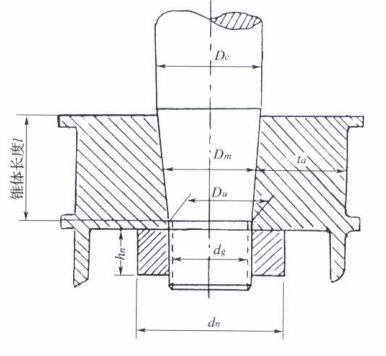
\includegraphics[width=2.5in]{figure/nut}
			\caption{锥体连接螺母}
			\label{fig:nut}
		\end{figure}
	\item 舵叶内的承座在其中点处的厚度应不小于锥体平均直径的0.25倍. 承座与垂直隔板和水平隔板应有良好的连接.
	\item 舵杆和舵柄的有键锥形连接可参照上述要求.
\end{enumerate}

\subsubsection{舵承}
	采用滑动轴承, CCS《钢质海船入级规范》关于舵杆、舵销及舵轴的滑动轴承的要求如下:
	\begin{enumerate}
		\item 轴承应有足够润滑, 其支撑面积$A_{b}(mm^2)$即支撑面的长度乘以直径之值, 应不小于按下式计算所得之值:
		\begin{equation}
			A_{b}=\frac{P}{[P]}
		\end{equation}
		式中:P--轴承的支持力(N)\\
		$[P]$--许用表面压力$(N/mm^2)$, 轴承衬套采用钢、青铜及热压青铜--石墨材料, 值为7.\\
		上舵承支持力$P_{u}=110219.458N, A_{bu}=15745.64mm^2$.\\
		下舵承支持力$P_{d}=218662.691N, A_{bd}=31237.53mm^2$.
		\item 承面长度和直径之比应不大于 1.2, 不妨取1.
		\item 金属轴承的径向间隙$\delta(mm)$应不小于下式计算所得之值:
		\begin{equation}
			\delta=\frac{d}{1000}+1
		\end{equation}
		式中:$d$--支承面的直径(mm).\\
		上舵承支承面直径$d_{u}=120mm$,长度$l_{u}=120mm$,径向间隙$1.12mm$.
		下舵承支承面直径$d_{d}=240mm$,长度$l_{u}=240mm$,径向间隙$1.24mm$.
	\end{enumerate}
	舵承表面压力计算, 计算时暂不计径向间隙:\\ \\
上舵承表面压力$=\frac{P_{u}}{2\pi d_{u}l_{u}}=1.218N/mm^2$.\\ \\
下舵承表面压力$=\frac{P_{d}}{2\pi d_{d}l_{d}}=0.604N/mm^2$.\\
\section{舵机功率}
描出力矩-角度点并进行六次多项式拟合,得曲线如图\ref{fig:power}所示, 表达式如式\ref{equ:malpha}所示:
\begin{equation}\label{equ:malpha}
	M(\alpha)=0.0001492\alpha^6 - 0.02077\alpha^5 + 1.027\alpha^4 - 23.06\alpha^3 + 281.8\alpha^2 + 33.11\alpha + 120.1
\end{equation}
求出上式关于$0-35^{\circ}$得积分为1196648.359375.\\

\begin{figure}
	\centering
	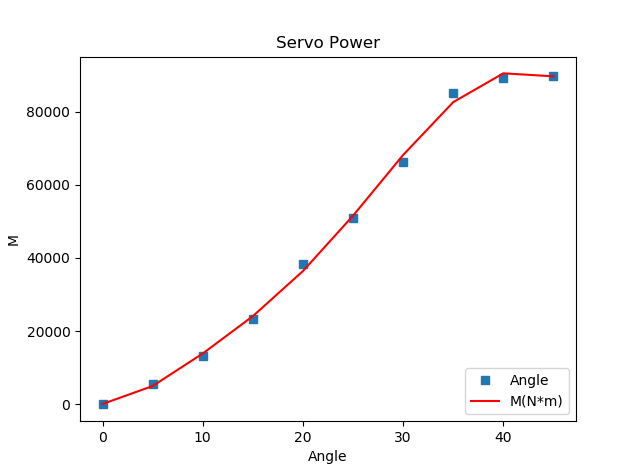
\includegraphics[width=3in]{figure/rudder_power}
	\caption{力矩-角度曲线}
	\label{fig:power}
\end{figure}
由技术规格书得从一舷$35^{\circ}$到另一舷$30^{\circ}$的转舵时间$\leq12s$.由式
\begin{equation}
	N_e=\frac{EK}{57.3t\eta}=6142.328095W
\end{equation}
式中:\\
$E$--转舵一定角度所需的功, 取$\pm35^{\circ}$, 即上述积分的二倍.\\
$K$--动力储备系数, 取1.5.\\
$\eta$--舵机型式影响系数, 取0.85.\\
$T$--转舵时间, 取12s.

\section{建议}
\begin{enumerate}
	\item 过程中有一些参数不明确, 如舵伴流系数, 倒车速度等, 希望老师可以总结出一张完整的参数表.
	\item 把一些常见错误总结出来, 事先发给学生, 避免学生在不必要的错误中耗费太多时间.
	\item 如果能整理出几份不同设计舵的标准流程就好了.
\end{enumerate}

\label{last}
\end{document}